\subsection{Analisis de topologias}

Se analizaron ambas topologias canonicas de realimentacion positiva/negativa, se plantearon ecuaciones de nodos y mediante el modulo SymPy de PYTHON se consiguieron las funciones de transferencia para cada una.

\subsubsection{Bicuadratica de Realimentacion positiva (Sallen-Key)}

\begin{figure}[H]
    \centering
    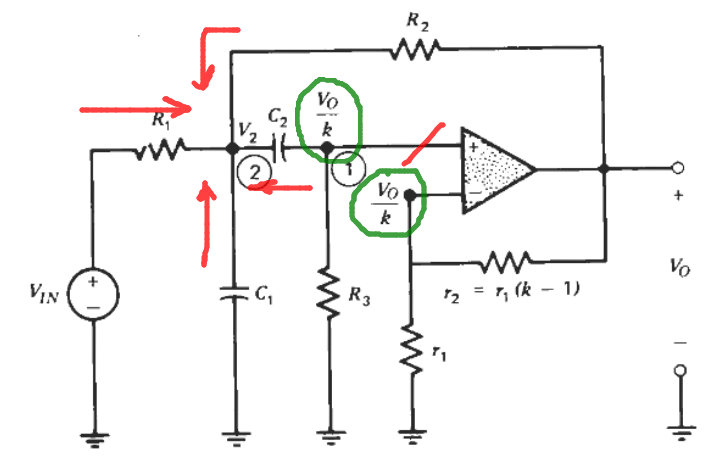
\includegraphics[scale=.5]{Secciones/Circ1/img/sallenKeyBP.png}
    \caption{Topologia de realimentacion positiva (Sallen-Key BP).}
    \label{c1}
\end{figure}

\noindent $>>$ \texttt{Considerando un amplificador ideal de ganancia k, planteando corrientes en los nodos y teniendo en cuenta que las corrientes por C2 y R3 son iguales, se llego a las ecuaciones:
}

\begin{align*}
    V_2 \left(C_{1} s + C_{2} s + \frac{1}{R_{2}} + \frac{1}{R_{1}}\right) - \frac{V_o}{R_{2}} - \frac{V_i}{R_{1}} - \frac{C_{2} V_o s}{k} = 0 \\
    \frac{Vo \left(C_{2} s + \frac{1}{R_{3}}\right)}{k} - C_{2} V_2 s = 0 
\end{align*}
    
\noindent $>>$ \texttt{Mediante PYTHON se resolvio para Vo/Vi y se obtuvo la funcion de transferencia del filtro:}

\begin{equation}\label{posFT}
    G = \frac{\frac{k}{C_{1} R_{1} }s}{s^{2} + s \left(\frac{1}{C_{2} R_{3}} + \frac{1}{C_{1} R_{3}} - \frac{k}{C_{1} R_{2}} + \frac{1}{C_{1} R_{2}} + \frac{1}{C_{1} R_{1}}\right) + \frac{1}{C_{1} C_{2} R_{2} R_{3}} + \frac{1}{C_{1} C_{2} R_{1} R_{3}}}
    = \frac{k_1 s}{s^{2} + a_1 s + b_1}
\end{equation}

\subsubsection{Bicuadratica de Realimentacion negativa}

\begin{figure}[H]
    \centering
    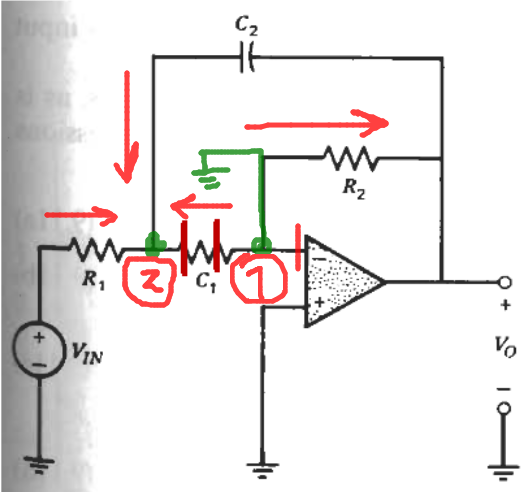
\includegraphics[scale=.5]{Secciones/Circ1/img/negBiquadBP.png}
    \caption{Topologia de realimentacion negativa, BP (corregido esquema del Daryanani).}
    \label{pv1}
\end{figure}

\noindent $>>$ \texttt{Planteando las ecuaciones de corriente para los nodos 1 y 2, y considerando al amplificador como ideal por lo que V1=0:}

\begin{align*}
    V_2 \left(C_{1} s + C_{2} s + \frac{1}{R_{1}}\right) - \frac{V_i}{R_{1}} - C_{2} V_o s = 0 \\
    - C_{1} V_2 s - \frac{V_o}{R_{2}} = 0
\end{align*}

\noindent $>>$ \texttt{Mediante PYTHON se resolvio para Vo/Vi y se obtuvo la funcion de transferencia del filtro:}

\begin{equation}\label{negFT}
    G = - \frac{\frac{1}{C_{2} R_{1}}s}{s^{2} + s \left(\frac{1}{C_{2} R_{2}} + \frac{1}{C_{1} R_{2}}\right) + \frac{1}{C_{1} C_{2} R_{1} R_{2}}}
    = \frac{k_2 s}{s^{2} + a_2 s  + b_2}
\end{equation}
